\documentclass[a4paper,landscape,usenames,dvipsnames,class=minimal,border=0pt]{standalone}
  \usepackage[margin=2.5cm]{geometry}
  \usepackage{tikz}
  \usepackage{pdfpages}
  \usetikzlibrary{matrix,
                 shapes,
                 calc,
                 intersections,
                 chains,
                 arrows,
                 arrows.meta,
                 scopes
  }

\pagestyle{empty}


\begin{document}

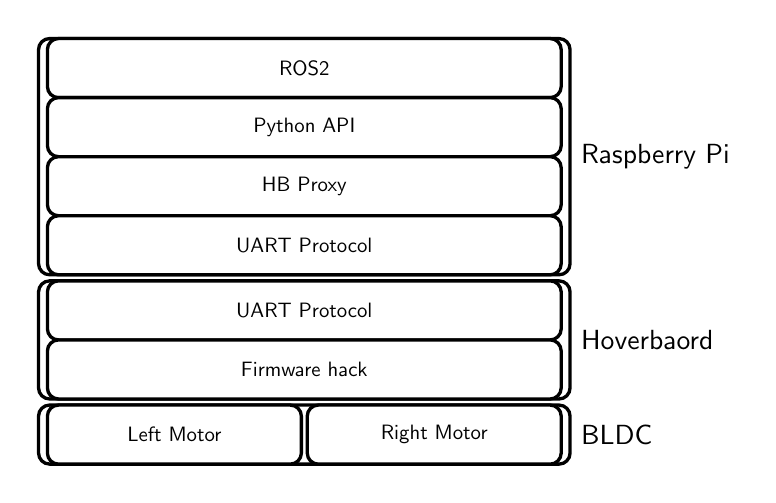
\begin{tikzpicture}[
      scale=0.75,
      node distance=1mm,
      layer/.style={
                scale=0.75,
                rectangle,
                rounded corners,
                draw=black,
                very thick,
                text centered,
                text width=2.5cm,
                minimum height=10mm,
                minimum width=90mm,
                fill=white
                },
      every node/.style={font=\sffamily}
]

\matrix [row sep=1, column sep=1]
{
  \node[layer, minimum height=40mm, label=right:Raspberry Pi] (rpi) {}; \\ 
  \node[layer, minimum height=20mm, label=right:Hoverbaord] (gd32f130) {}; \\
  \node[layer, label=right:BLDC] (hw) {}; \\
};

\node[layer, minimum height=10mm, minimum width=87mm] () at ($ (rpi) + (0,1.5) $) {ROS2};
\node[layer, minimum height=10mm, minimum width=87mm] () at ($ (rpi) + (0,0.5) $) {Python API};
\node[layer, minimum height=10mm, minimum width=87mm] () at ($ (rpi) + (0,-0.5) $) {HB Proxy};
\node[layer, minimum height=10mm, minimum width=87mm] () at ($ (rpi) + (0,-1.5) $) {UART Protocol};

\node[layer, minimum height=10mm, minimum width=87mm] () at ($ (gd32f130) + (0,0.5) $) {UART Protocol};
\node[layer, minimum height=10mm, minimum width=87mm] () at ($ (gd32f130) + (0,-0.5) $) {Firmware hack};

\node[layer, minimum height=10mm, minimum width=43mm] () at ($ (hw) + (-2.2,0.0) $) {Left Motor};
\node[layer, minimum height=10mm, minimum width=43mm] () at ($ (hw) + (2.2,0.0) $) {Right Motor};

\end{tikzpicture}

\end{document}
